In this chapter planning and work-flow regarding Sprint 1 will be described. 
All from setting  goals to implementation and testing. On the end team will evaluate whole sprint and try to answer the following questions: What went well? What could be improved? What should we start doing?  


\section{Sprint Planning}
After assembling all the tools in Sprint 0, team decided to start with the implementation of the core modules.
As teams understanding of task improved, they were able to come up with user stories from the perspective of user, customer, developer and a student.
All user-stories were given to the customer so they can be prioritized. 
All but user-stories concerning team school obligations, like writing project plan, minutes, meetings with supervisor and attending lectures.
Team decided to have school tasks as a user stories so time can be better tracked.
School user-stories were mandatory and already added as a user-stories of sprint 1.
On Monday 02.09.2013. team had meeting with the customer where time needed for every user story were estimated.
Result of that meeting was list of rest of the user-stories for sprint 1.

For the documentation part, team made a document "project plan". 
Supervisor wanted these sections to be integrated in the project report instead. 
Therefore team decided to make the content for the report, and to make the general structure for it. 
Also integrate the parts previously written in the project plan into the project report. 
Team also planed to add the additional sections that were missing.

\subsection{Duration}
This Sprint will be 2 weeks long. From 02.09.2013 to 15.09.2013.
The team agreed on the date for presentation and showing the running demo -- Thursday 12.09.2013.
Estimated velocity is 240h since team agreed on 30 working hours per person per week.

\subsection{Sprint 1 User-stories}

\subsubsection*{Implementation}
All the functional requirements for sprint 1 are presented in table \ref{tab:sprint1stories}
\LTXtable{\textwidth}{sprint1/stories.tex}

\subsubsection*{Documentation}
All the documentation stories for sprint 1 are presented in table \ref{tab:sprint1Documentationstories}
\LTXtable{\textwidth}{sprint1/storiesDocumentation.tex}

\subsubsection*{Project management}
All the project management stories for sprint 1 are presented in table \ref{tab:sprint1storiesProcess}
\LTXtable{\textwidth}{sprint1/storiesProcess.tex}

% hous all in total: Estimated: 45+84+89=218 Spent: 37+96+81=214

\section{Sprint Goal}

Team's goal for this Sprint is to deliver working demo over core client-server module.
This includes registering services, listening for the client and sending simple signals to the client from the server application.
Scanning for the services, connecting, receiving signals and play commands on the client.
Establishing simple communication protocol and implementing Test-Flight in both applications, the server and the client.

The goal for the documentation is to have a good structure for the report, and integrate the project plan in the project report. It must be evaluated whether to write more of remove sections after integrating. The goal is also to finish the chapters that are a part of this sprint, which means we need to finish the sprint 0 chapter, and of course write the sprint 1 chapter.

\section {Research}
In this section all research connected to finishing user-stories, taken before work on actual code, will be described, as well as a decisions team made in order to successfully finish sprint 1.

\subsection{Bonjour software}
The first research of technologies that could help with achieving client-server communication, without writing everything from scratch, was Bonjour software. 
It is a group of technologies that includes service discovery, address assignment, and hostname resolution. 
Bonjour locates devices such as printers, other computers, and the services that those devices offer on a local network using multicast Domain Name System (mDNS) service records.
It is the Apple's implementation of Zero configuration network (Zeroconf).
Aldo good and very useful tool it is not supported on Android, and since Android is the platform chosen for the DigialLighter product further research must have been carried out. 
Zeroconf software written in Java with similar set of services as Bonjour seemed to be the best option.

\subsection {Zero configuration (Zeroconf)}
Zeroconf is a methodology and a set of special technologies that automatically create a usable wireless network based on the Internet Protocol Suite (TCP/IP) when computers or network peripherals are interconnected. 
It does not require manual operator intervention or special configuration servers.
It is assembled of technologies that includes service discovery, addressing assignment, and host name resolution.


\subsection{JmDNS library}
Further research brought JmDNS. 
Java implementation of multi-cast DNS that can be used for service registration and discovery in Local Area Network. 
It works on most JDK1.6 compatible Virtual Machines, it comes as a library and it is easy to integrate with Android. 
JmDNS fulfill all of the expectations, but while learning about it, team found that Android itself have built in Nestwork Service Discovery(NSD) that do the same thing.

\subsection{Android Network Service Discovery (NSD)}
NSD is supported from API version 16. 
It allows users to identify other devices on the local network, register services, broadcast connection information, scan for registered services and connect.
Even with API limitation it is a part of Android platform, no third part libraries are needed, it will evolve with Android and therefore always be working.
Min API version was not of concern to the customer, so team made a decision of using Android Network Discovery(NSD) for client-server core module.

\section{Architecture}
For the core communication and organization of our product the client-server architecture was selected as shown in figure \ref{fig:sprint1_arhitecture}.
Choosing this architecture was very intuitive to do as the project should consist of two applications and overall tasks should be partitioned. 
Client application should be able to light up different sequences of lights depending on server command signals.
And server application should be responsible for awaiting incoming clients connections, mapping clients to the grid and providing command play signals to the clients by broadcast.
Communication should be established over wireless network using same router for both applications, the user and the server, and without need for third party server nor Internet connection.

\begin{figure}[H]
	\centering
		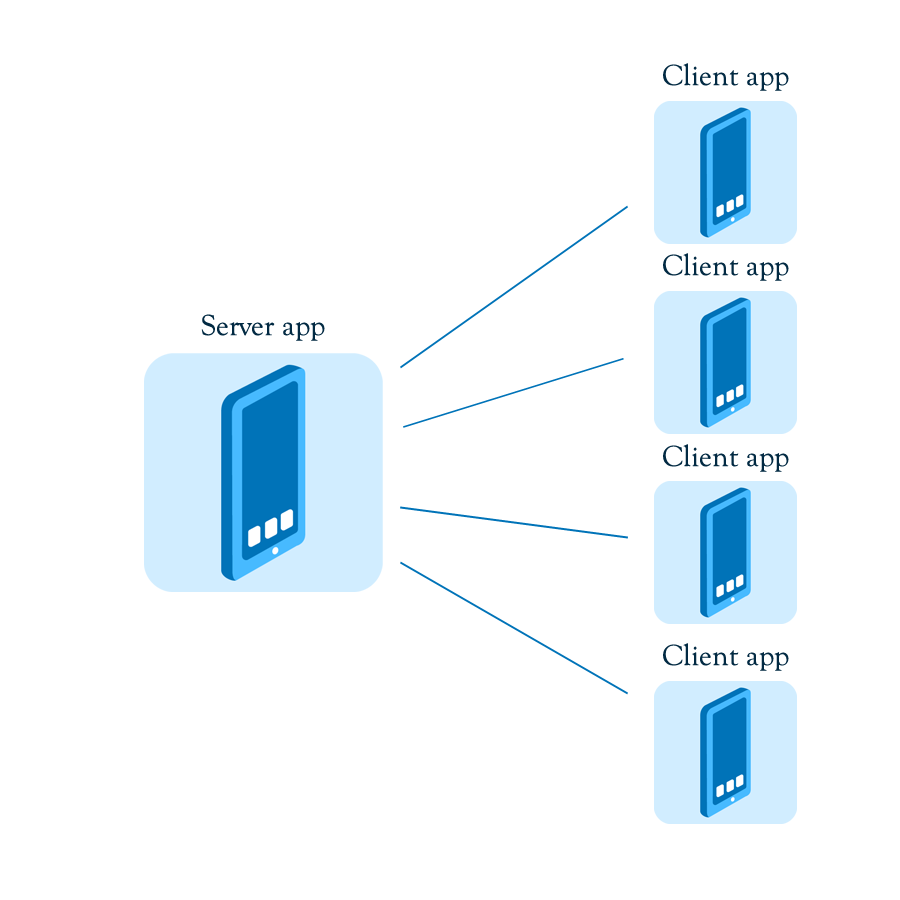
\includegraphics[width=7cm]{sprint1/arhitecture.png}
	\caption{Client-server architecture}
	\label{fig:sprint1_arhitecture}
\end{figure}

For illustrating software architecture "4+1" architectural model view\ref{fig:4+1} will be used.

\subsection{Logical View}
Figure \ref{fig:class_diagram_client} gives an overview of the client class structure and collaboration. As planed client have all of the functionality covered by user stories. 

\begin{figure}[H]
	\centering
		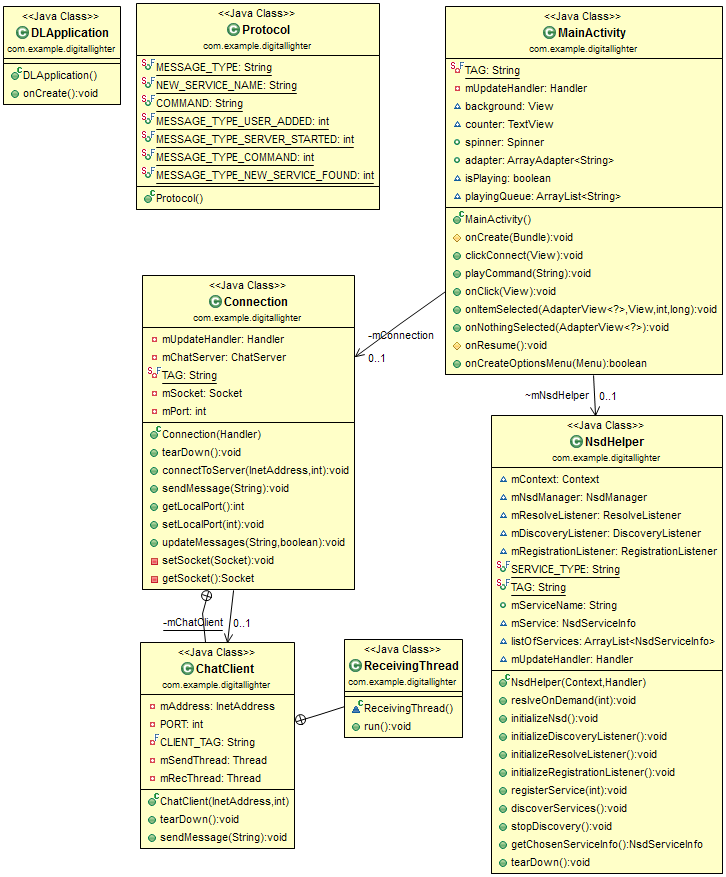
\includegraphics[width=10cm]{sprint1/class_diagram_client.png}
	\caption{Sprint 1 client class diagram}
	\label{fig:class_diagram_client}
\end{figure}

Figure \ref{fig:class_diagram_server} gives an overview of the server class structure and collaboration. Separated thread "ServerThread" for incoming clients was made to optimize server. Sending command signals is also moved from UI thread to "SendingThread" in order to make application more responsive.

\begin{figure}[H]
	\centering
		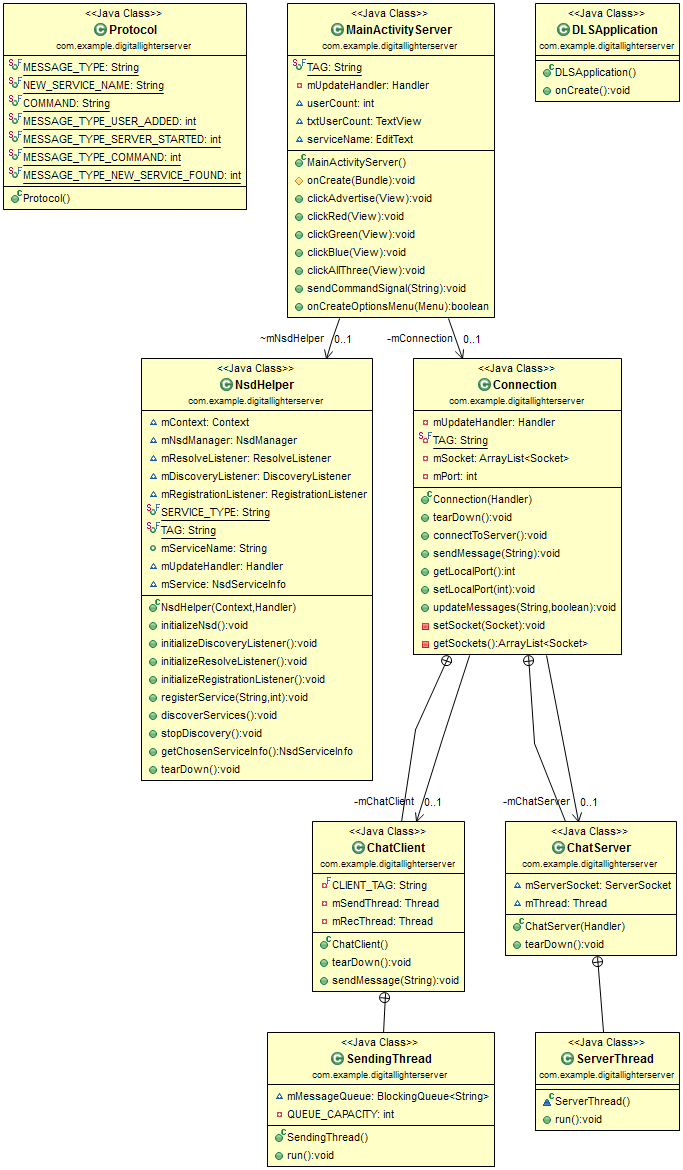
\includegraphics[width=10cm]{sprint1/class_diagram_server.png}
	\caption{Sprint 1 server class diagram}
	\label{fig:class_diagram_server}
\end{figure}

In the sequence diagram \ref{fig:sprint1_communication} it is showed how applications can be used. It gives an idea of how the data flows between different parts of the system when it is up and running.

\begin{figure}[H]
	\centering
		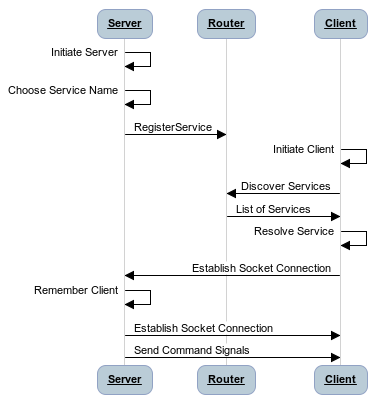
\includegraphics[width=9cm]{sprint1/communication.png}
	\caption{Sprint 1 Communication}
	\label{fig:sprint1_communication}
\end{figure}

\subsection{Physical View}
The deployment diagram, displayed in \ref{fig:deployment_diagram} describes the system architecture focusing on the large components and their connections.

\begin{figure}[H]
	\centering
		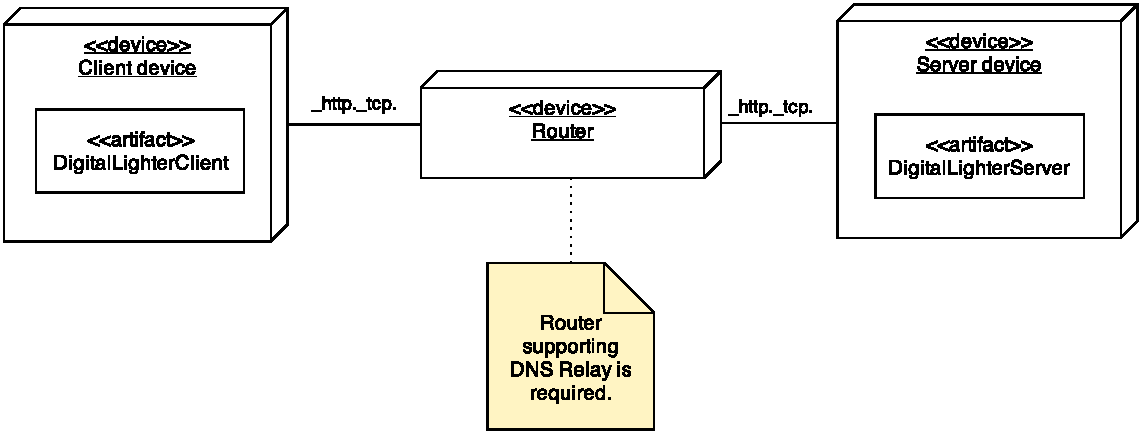
\includegraphics[width=15cm]{images/deployment-diagram-sprint1}
	\caption{Deployment diagram}
	\label{fig:deployment_diagram}
\end{figure}

\paragraph{Client}
is the application that runs on audience Android device. It is able to discover available services, connects to the one and receives command signals from the server. After receiving commands the client is able to flash screen according to given signal.

\paragraph{Router}
is inevitable part of client-server communication since project is based on wireless network and zeroconf technologies. In order to support all the demands demands it have to include a DNS relay service. The relay embraces storing of service names and allows look-up stored data to the clients.

\paragraph{Server}
is the application that runs on manager's Android device. It have to register service that it provides at router DNS table. Once registered it have to be able to listen for the clients and broadcast command signals to them.


\section{Implementation}

In this sprint most of the work have be done on time. Actual progress was not ideal, but team managed to finish all of the goals that have been set on the beginning of the sprint.
Actual burn down chart can be seen on figure \ref{fig:Burn1 } that is generated by team  management tool TargetProcess 3 \ref{subsec:targetProcessToolDescription}.  

\begin{figure}[H]
	\centering
		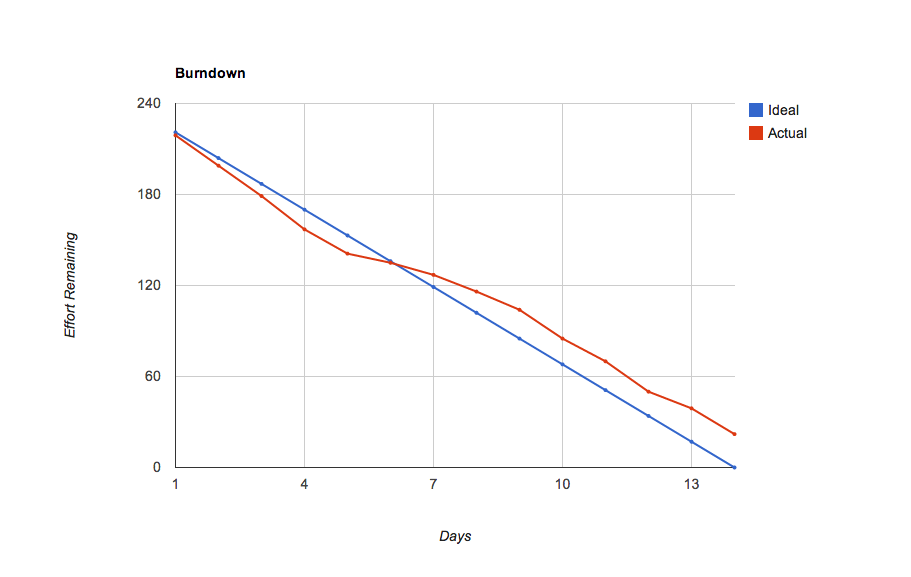
\includegraphics[width=18cm]{sprint1/BurndownSprint1.png}
	\caption{Burn down chart.}
	\label{fig:Burn1 }
\end{figure}


\section{Occurring risks}
The risk table 3.3, taken from the risk management section in the planning chapter, shows the risks that can occur this project. 
For this sprint most of them did not occur. 
This is because the hardest technical parts, which is the image processing, is not scheduled until the upcoming sprints. 

The user stories for this sprint was very clear, and the customer did not change any of them in the last minute. The team overestimated some of the user stories, so we did not experience pressure with the time frame. 

The first risk in the risk table describes team members being sick. This did not occur, but what did occur was that that some of team members had to be absent in some of the working hours. 
The team solved this by having these team members work more independently, and with more flexible hours.  

For now only Android 4.1 adds support for multicast DNS-based discovery.
One of the risks is that Android will not make it available for lower platforms.
In that case a bit over 50\% of the devices will not be supported as shown on the figure \ref{fig:Platform_chart }, and future development of our prototype will require some of the third part libraries we discovered in prestudy or similar.
Supporting lower platforms in the future, or not, is however never stated in any official document of the Android documentation.

\begin{figure}[H]
	\centering
		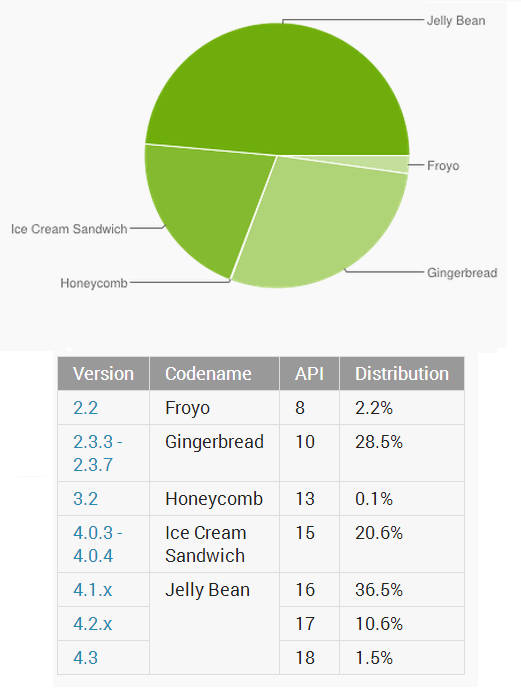
\includegraphics[width=10cm]{sprint1/android_platform_chart.png}
	\caption{Data collected during a 7-day period ending on October 2, 2013. 
	Any versions with less than 0.1\% distribution are not shown.}
	\label{fig:Platform_chart }
\end{figure}

\section{Customer feedback}

\section{Retrospective}
In this section the team will take a look back at sprint 1, and review this sprint. The focus will be on what went well, and goal we achieved. Another focus will also be what we could have done differently, and of course and learn from what we could have done differently.

\subsection{What went right}
For the implementation part the sprint 1 goals were reached. The working demonstration video over core client-server module was delivered. The server side registers services, listens for the client, and sends simple  signals. The client is scanning for the services, connecting, receiving signals and play commands on the client. The customer was very satisfied with the video, and suggested recording our future prototypes as well. Besides this we reached the goal to implement Test-Flight in both applications. We also reached the milestone, Obedient client -- Prototype 1.

For the documentation the work done is in the report is good. The report is better structured now, and it actually looks like a report, which is good. The supervisor liked the structure as well. A lot of sections were added when the team integrated the project plan in the report, so that the introduction, the preliminary studies and the planning chapter would be as complete as possible. In for example the preliminary studies chapter the team has not written all of the studies about the image processing part yet, because the team will research this more in later sprints.

\subsection{What to improve}
The sprint planning in this sprint could have been better. Some of the implementation user stories were over estimated. To solve this better till next time the team should spend more time doing the planning poker. This makes sure that everyone understands the task better. 

The structure of the report is good, but the number of chapters wuold probably have to be reduced. The supervisor suggested to move the test plan chapter in the planning chapter, since it was such a small chapter. The supervisor also wanted the team to work more with the requirements chapter. There should be a better connection between the user stories and the requirements.


Another con this sprint was that when the product was tested on the mobiles there were problems with the network. Since the mobiles were on different subnets, the client could not find the server. We had to borrow a router and bring with us to be able to test. 

